\section{Libras}

A Língua Brasileira de Sinais (LIBRAS) é um idioma que possui uma estrutura gramatical própria, contendo particularidades 
idiomáticas e regionalismos, que se assemelham ao sotaque ou as gírias da língua portuguesa. Cada país fala uma língua diferente, 
nos Estados Unidos, por exemplo, é utilizada a \textit{American Sign Language} (ASL), com seu vocabulário derivado da Língua 
Francesa de Sinais há 180 anos, e LIBRAS, também é derivada da Língua Francesa de Sinais. Embora a Inglaterra e Estados Unidos tenham inglês como idioma principal, as 
línguas de sinais são completamente diferentes. Isto também serve para o português e LIBRAS, onde LIBRAS não é o português 
sinalizado.\cite{Comunicacao}.

Para \citeonline{Zieren2006b}, em linguagens de sinais em geral, a informação é gerada por combinação dos seguintes fatores: 
configuração de mão; posicionamento da mão ou ponto de articulação; movimento; orientação (direção do sinal); e expressão facial e 
corporal.
Alguns sinais podem ser distinguidos pela configuração de mão somente, e em outros casos é a combinação de todos os fatores que 
devem ser executados evitando uma interpretação ambígua.

Em alguns casos, não existem sinais que expressem siglas, nomes, ações ou gírias. Então é desenvolvido de um alfabeto manual 
(vide Figura \ref{fig:alfabeto}) que é constituído de configuração de mão que representa uma letra e, em alguns casos, um 
movimento. Através da datilologia ou soletração digital, este alfabeto é utilizado para expressar essas palavras para as quais não 
existe um sinal equivalente  \cite{PorUmaGramatica}.


\begin{figure}[H]
	\centering
	\vspace{4mm}
	\caption{Alfabeto manual de LIBRAS}
	\label{fig:alfabeto}
	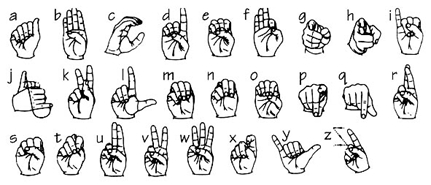
\includegraphics[scale =0.5]{imagens/Alfabeto_Libras.jpeg}
	\caption*{Fonte: \citeonline{Comunicacao}.}
\end{figure}


Como a Figura \ref{fig:CERTO} apresenta, a palavra "certo" que em datilologia exige cinco gestos para definir o  seu significado, 
enquanto utilizando o sinal existente, pode ser definida apenas com um gesto.
\begin{figure}[H]
	\vspace{4mm}
	\centering
	\caption{Comparação entre datilologia e sinal pronto da palavra certo}
	\label{fig:CERTO}
	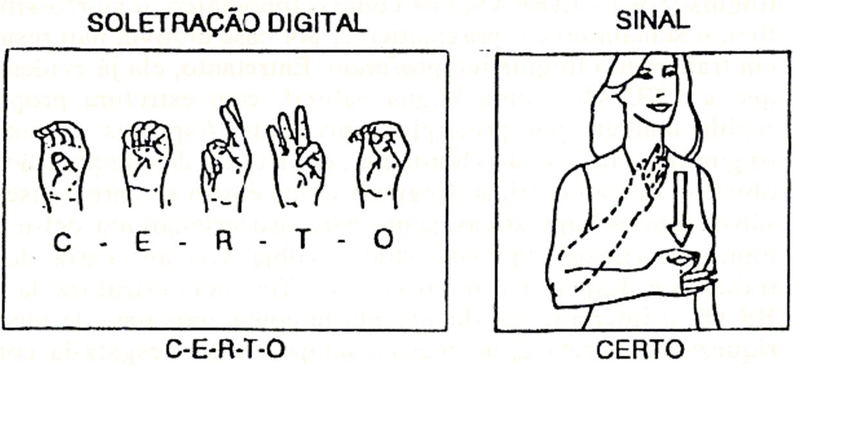
\includegraphics[scale=0.4, trim={0 1cm 2cm 0}, clip]{imagens/Certo}
	\caption*{Fonte: \citeonline[p. 22]{PorUmaGramatica}.}
\end{figure}

Existem ainda, muitas limitações no processo de comunicação, entre surdos e ouvintes em ambientes como
trabalho, escolas, universidades e no próprio ambiente familiar de surdos, provocando um distanciamento
\cite{jogoslibras}, que podem ser minimizadas, gradativamente, pelo
uso de objetos de aprendizagem \cite{ferramentas}.


Conforme \citeonline{martinsEmatos}, as tecnologias podem facilitar a inserção comunicativa dos surdos, assim como para os ouvintes, com o uso
frequente, por exemplo, das redes sociais, que apesar de primar pelo lazer, possibilitam um maior contato com o
português, uso de dicionários on-line e os objetos de aprendizagem (hipermídias, softwares, jogos etc), permitindo
aos surdos, o contato com materiais mais interessantes e atrativos.


